%!TEX program = xelatex
\documentclass[10pt]{beamer}
\usepackage{amsmath}

\numberwithin{figure}{section}
\usetheme[menuwidth={0.5\paperwidth}]{erlangen}
\setbeamercovered{transparent=20}
\setbeamerfont{frametitle}{series=\bfseries}
\usepackage[hyperref,UTF8,space]{ctex}

\hypersetup{colorlinks=false,
            colorlinks=black,
            pdfborder=100,
            citecolor=black}
% \usefonttheme{serif}
\setbeamerfont{block title}{series=\bfseries}
\usepackage{graphicx,texnames,mflogo,subfig}
\graphicspath{{./images/}}
\newcommand{\TIKZ}{Ti\textit{k}Z}
\renewcommand\contentsname{目录}
\newcommand{\pbf}[1]{\noindent\textbf{#1}}
\setcounter{tocdepth}{1}

\usepackage{fontspec}
\defaultfontfeatures{Mapping=tex-text}
\RequirePackage{xunicode}
\RequirePackage{xltxtra}
\setmainfont[Ligatures=TeX]{Minion Pro} %  (\textrm)
\setsansfont{Myriad Pro} %  (\textsf)
\setmonofont{Monaco}%Palatino Linotype
%-中文字体设置-%
\usepackage{xeCJK}
\setCJKmainfont[BoldFont={方正黑体简体},ItalicFont={方正楷体简体}]{方正楷体简体}
%方正书宋_GBK Adobe Song Std L华文中宋
\setCJKsansfont[BoldFont={方正黑体简体}]{方正中等线简体}
\setCJKmonofont{微软雅黑Monaco}
\XeTeXlinebreaklocale "zh"
\XeTeXlinebreakskip = 0pt plus 1pt

% \setCJKmonofont{Adobe Fangsong Std}
% \setCJKmainfont{Adobe }
\definecolor{god}{RGB}{184,134,11} %184,134,11
\usepackage{listings,relsize}
\lstset{% general command to set parameter(s)
language = [LaTeX]{TeX},
basicstyle=\scriptsize\ttfamily, % print whole listing small
keywordstyle=\color{god},
commentstyle=\color{gray}, % white comments
prebreak = \raisebox{0ex}[0ex][0ex]{\ensuremath{\hookleftarrow}},
backgroundcolor=\color{green!5},
stringstyle=\ttfamily, % typewriter type for strings
showstringspaces=false,
numbers=left, numberstyle=\tiny, stepnumber=1, numbersep=5pt, %
frame=shadowbox,
rulesepcolor=\color{gray},
columns=fullflexible,
extendedchars=\true,
texcsstyle=*\color{erlangenblue},
morekeywords={url,convert,bmeps,mkdir,for,do,in,ebb,label,caption,textwidth,centering,figure,graphicx,minipage,pspicture,psline,uput,color,psgrid,psarc,tikzpicture,draw,fill,coordinate,node,intersection of,LaTeX,PDFLaTeX,XeLaTeX},
moretexcs={subfloat,usepackage,DeclareGraphicsRule,DeclareGraphicsExtensions,graphicspath,includegraphics,SpecialCoor},
} %
\begin{document}

\title[\LaTeX{} 插图与绘图简介]{ \LaTeX{} \bfseries 插图与绘图简介}
\subtitle{China\TeX{} \bfseries 在线培训课程}
\author[ddswhu]{\small\sffamily 邓东升(\href{http://ddswhu.com/}{ddswhu}) \\{\color{erlangenblue}}}
\date{\today}
\institute{Fudan University\\
  \vspace{-0.2em}{\small School of Economics} }

\begin{frame}[plain]
\titlepage
\end{frame}


\begin{frame}{目录安排}
  \tableofcontents
\end{frame}
\section{引言}
\begin{frame}[c]\frametitle{引言}

西方学者常说:A picture is worth a thousand words。译作:一图胜千言,意思是说,一幅图形可以简单明确地表达很多错综复杂,千言万语都难以描述的信息。所以说一篇优秀的论文应该是图文并茂。

\LaTeX{} 的绘图功能比较简单,如使用 \LaTeX{} 相关的各种绘图宏包或者绘图工具比如:\MP、PSTricks、PGF (\TIKZ)等,借助这些工具我们可以画图非常复杂的图形,但缺点是不直观,命令繁琐,不易熟练掌握。

现在,通常是用 Matlab、R、Visio 等功能强大的绘图工具先把图形画好,然后插入到 \LaTeX{} 源文件中。

\end{frame}

\section[例子]{一个简单的例子}

\begin{frame}[c,fragile]\frametitle{一个简单的例子}
\noindent 需要插入的图片(logo.png)在我们的主文件夹内,我们使用 \lstinline{PDFLaTeX} 编译,图片的宽度为 0.3 * 文档宽度(\lstinline{\textwidth}),标题为``这是一个 LOGO'',为方便引用,我们设置标签为 ``fig:elegantlatex\_logo''。使用到的命令如下:

\begin{lstlisting}
\begin{figure}[htbp]
  \centering
  
\includegraphics[width=0.3\textwidth]{logo.png}
  \caption{这是一个 LOGO\label{fig:elegantlatex_logo}}
\end{figure}
\end{lstlisting}

\begin{figure}[htbp]
  \centering
  
\includegraphics[width=0.3\textwidth]{logo.png}
  \caption{这是一个 LOGO\label{fig:elegantlatex_logo}}
\end{figure}

\end{frame}


\section{位图与矢量图}

\begin{frame}[c]\frametitle{位图}

图形的存储格式很多,一般分为两大类:位图与矢量图,都是以数字形式存储,解释方法各不相同。
\vskip2ex

\pbf{位图(bitmap):} 也称点阵图,栅格图象,像素图。

\begin{itemize}
  \item 最小单位由像素(Pixel)构成的图,缩放会失真;
  \item 由像素阵列的排列来实现其显示效果的;
  \item 每个像素有自己的颜色信息,可操作对象为像素(HSB)。
  \item 每英寸所拥有的像素数目用 PPI(分辨率的单位)表示。
\end{itemize}

% 举个例子来说,位图图像就好比在巨大的沙盘上画好的画,当你从远处看的时候,画面细腻多彩,但是当你靠的非常近的时候,你就能看到组成画面的每粒沙子以及每个沙粒单纯的不可变化颜色。
\end{frame}

\begin{frame}[c]\frametitle{矢量图}

\pbf{矢量图(vector):} 也叫做向量图。

\begin{itemize}
  \item 由数学公式定义的线段和曲线组成;
  \item 纪录了元素形状及颜色的算法;
  \item 可以将其任意缩放和旋转,都不会失真;
  \item 矢量图与分辨率无关;
  \item 矢量图文件尺寸一般比较小
\end{itemize}
\end{frame}

\section[编译方式支持]{编译方式与图形格式}

\begin{frame}[c,fragile]\frametitle{编译方式与图形格式支持}

我们通常使用 \lstinline{LaTeX}、\lstinline{PDFLaTeX}、\lstinline{XeLaTeX} 编译源文件。各种编译方式下图形格式支持如下:

\begin{enumerate}
  \item \lstinline{LaTeX} 只支持 EPS、PS 图形文件;
  \item \lstinline{PDFLaTeX} 支持 PNG、PDF、JPEG 格式图形文件,不支持 EPS;
  \item \lstinline{XeLaTeX} 直接支持 BMP、JPEG、PNG、EPS 和 PDF。
\end{enumerate}

\begin{alertblock}{注意事项:}
在使用 \lstinline{PDFLaTeX} 时,如果要插入 EPS,可以先把 EPS 转化为其他格式(比如 PDF、JPG),或者在导言区加载 \lstinline{epstopdf}。
\end{alertblock}

\end{frame}


\section[格式转化]{图形格式转化与灰度图}
\begin{frame}[c,fragile]\frametitle{批量得到 eps 图档}
虽然「\LaTeX{} 只能识别 EPS 格式的图档」是多年的误传,但是仍有许多杂志和期刊只接受 EPS 格式的图档。所以,尽管在日常使用中,我们很少会用到 EPS 格式,但是有时候不得不用。

在现在的 TeX 发行版中,一般都带有一个 bmeps 的小程序,它能将 PNG,JPEG 和 BMP 等格式的位图转换成 EPS 格式的图档。以 JPEG 格式为例,批处理命令(来源于小 L)如下:
\begin{lstlisting}
for /f %%i in ('dir /b *.jpg') do (
    @echo %%i
    bmeps -c %%i %%~ni.eps
    @echo Finished
    )
\end{lstlisting}

\href{http://liam0205.me/2014/08/21/bitmap-convert-to-eps-batch/}{\textbf{点击此处有惊喜!}}

\end{frame}

\begin{frame}[c,fragile]\frametitle{使用 ImageMagick 得到灰度图}
在实际写作中,我们更可能需要用到灰度图,这里推荐使用 ImageMagick(需要自行安装),这个一个非常强大的图形处理软件。单个图片的转化使用 \lstinline{convert 1.jpg -colorspace Gray 1_out.jpg}。\\
送福利时刻:

\begin{lstlisting}
mkdir out
for %%B in (*.jpg) do convert "%%B" -colorspace Gray "out/%%B"
\end{lstlisting}

\href{http://blog.sina.com.cn/s/blog_630306a50101cp5c.html}{\textbf{戳这里有奖!}}

\end{frame}

\section[插图详解]{插入图形}
\subsection{BoundingBox}
\begin{frame}[c,fragile]\frametitle{BoundingBox 问题}

由于历史原因,\lstinline{LaTeX} 编译程序不能提取 JPEG、PNG 等点阵图形的尺寸信息,所以它在处理这些图形文件时需要范围框 。\lstinline{PDFLaTeX} 和 \lstinline{XeLaTeX} 的用户可以跳过本节内容。

EPS 的范围框如下,其中前两个参数是图形左上角的坐标 (通常就是原点),后两个参数是右下角的坐标,缺省长度单位是 bp。
\begin{lstlisting}
%!PS-Adobe-2.0 EPSF-2.0
%%BoundingBox: 0 0 510 284
\end{lstlisting}

有了范围框,\lstinline{LaTeX} 在编译源文件时就可以为插图预留空间;它输出的 DVI 只记录图形尺寸和文件名,因为具体的图形处理由后面的驱动负责。找不到范围框时,\lstinline{LaTeX} 就会报错,

\begin{lstlisting}
! LaTeX Error: Cannot determine size of graphic in fig.png
(no BoundingBox).
\end{lstlisting}

\end{frame}

\begin{frame}[c,fragile]\frametitle{解决 BoundingBox 方案一}
在使用 \lstinline{LaTeX} 编译的时候,比较好解决 BoundingBox 缺失问题的方法是使用 \lstinline|bmpsize| 宏包(谢谢小 L),使用方法如下:
\begin{lstlisting}
\documentclass{article}
\usepackage[dvipdfm]{graphicx}
\usepackage{bmpsize}
\begin{document}


\includegraphics{logo.png}

\end{document}
\end{lstlisting}

\end{frame}

\begin{frame}[c,fragile]\frametitle{解决 BoundingBox 方案二}

有两种方法可以为点阵图形提供范围框:
\begin{enumerate}
  \item 准备一个单独的范围框文件;
  \item 插入图形时加范围框参数。
\end{enumerate}

使用 TeX 发行版中的 \lstinline{ebb} 小工具可以获取 BoundingBox 信息,比
如下面的命令会生成一个 1.bb 文件。
\begin{lstlisting}
ebb 1.jpg
\end{lstlisting}

\pbf{使用范围框文件:}
\begin{lstlisting}
\DeclareGraphicsRule{.jpg}{eps}{.bb}{}

\includegraphics[width=0.6\textwidth]{1.jpg}
\end{lstlisting}
\pbf{使用范围框参数:}
\begin{lstlisting}

\includegraphics[bb=0 0 300 200,width=0.6\textwidth]{1.jpg}
\end{lstlisting}

\end{frame}

\subsection{基本命令}
\begin{frame}[c,fragile]\frametitle{插图基本命令}
我们插图一般使用到的宏包是 \lstinline{graphicx},插图的基本命令如下:
\begin{lstlisting}
\usepackage{graphicx}
\includegraphics[width=0.5\textwidth]{fig.png}
\end{lstlisting}

使用 \lstinline{LaTeX} 时,如果事先没有生成 .bb 文件的话,需要或加范围框参数。\lstinline{PDFLaTeX} 和 \lstinline{XeLaTeX} 不需要该参数。
\end{frame}
\subsection{图形操作}

\begin{frame}[c,fragile]\frametitle{图形操作参数说明}

\lstinline{\includegraphics} 命令有一些参数选项可以用于缩放、旋转、裁剪等图形操作,简要说明如下:
\begin{columns}
\begin{column}{0.64\textwidth}
\begin{itemize}
  \item \lstinline{width=x},\lstinline{height=y}:宽度和高度,绝对尺寸,可用任意长度单位;
  \item \lstinline{scale=s}:缩放比,相对尺寸,使用上面参数与缩放时,绝对尺寸起作用;
  \item \lstinline{keepaspectratio}:保持长宽比;
  \item \lstinline{angle=a}:旋转角度;
  \item \lstinline{origin=hv}:旋转中心,(参考右图);
  \item \lstinline{trim=l b r t}:左下右上裁剪值;
\end{itemize}
\end{column}
\begin{column}{0.36\textwidth}
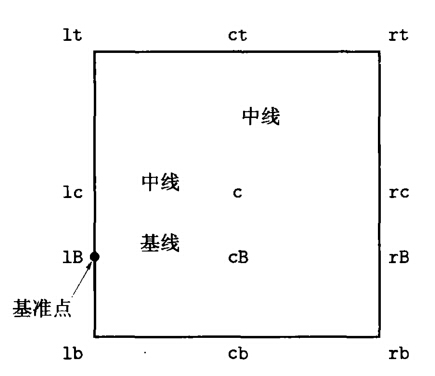
\includegraphics[width=1.1\textwidth]{origin.jpg}
\end{column}
\end{columns}

\end{frame}

\subsection{文件名与路径}
\begin{frame}[c,fragile]\frametitle{文件名与路径}
若想省略文件后缀或路径名,可以使用下面的命令:
\begin{lstlisting}
\DeclareGraphicsExtensions{.eps,.mps,.pdf,.jpg,.png}
\DeclareGraphicsRule{*}{eps}{*}{}
\graphicspath{{C:/secret_garden/}}
\graphicspath{{./img/}}
\graphicspath{{first_dir/}{second_dir/}{third_dir/}}
\end{lstlisting}
\pbf{说明如下:}

\begin{enumerate}
  \item 第一行指定后缀列表让编译程序自行查找;
  \item 第二行指出未知后缀的都是 EPS;
  \item 后三行设置缺省搜索路径,分别使用了绝对路径、相对路径、多个路径。
\end{enumerate}

\end{frame}
\subsection{Figure 环境}
\begin{frame}[c,fragile]\frametitle{figure 环境}
插图通常需要占据大块空间,所以在文字处理软件中用户经常需要调整插图的位置。figure 环境可以自动完成这样的任务;这种自动调整位置的环境称作浮动环境 (float),还有一个常用到的浮动环境是 table。

\begin{columns}
\begin{column}[c]{0.5\textwidth}
\begin{lstlisting}
\begin{figure}[htbp]
\centering

\includegraphics{myphoto.jpg}
\caption{有图有真相}
\label{fig:myphoto}
\end{figure}
\end{lstlisting}
\end{column}
\begin{column}[c]{0.5\textwidth}
\begin{figure}[htbp]
\centering

\includegraphics[width=0.5\textwidth]{myphoto.jpg}
\caption{有图有真相\label{fig:myphoto}}
\end{figure}
\end{column}
\end{columns}

\end{frame}

\subsection{插入多图}

\begin{frame}[c,fragile]\frametitle{并排摆放,共享标题}
当我们需要两幅图片并排摆放,并共享标题时,可以在 figure 环境中使用两个 \lstinline{\includegraphics} 命令:
\begin{columns}
\begin{column}[c]{0.55\textwidth}
\begin{lstlisting}
\begin{figure}[htbp]
\centering

\includegraphics{leftfoot.png}

\includegraphics{rightfoot.png}
\caption{向左走向右走}
\end{figure}
\end{lstlisting}
\end{column}
\begin{column}[c]{0.41\textwidth}
\begin{figure}[htbp]
\centering

\includegraphics[scale=0.4]{leftfoot.png}

\includegraphics[scale=0.4]{rightfoot.png}
\caption{向左走向右走}
\end{figure}
\end{column}
\end{columns}

\end{frame}

\begin{frame}[c,fragile]\frametitle{并排摆放,各有标题}
如果想要两幅并排的插图各有自己的标题,可以在 figure 环境中使用两个 minipage 环境,每个里面插入一幅图。不用 minipage 的话,因为插图标题的缺省宽度是整个行宽;两幅插图就会上下排列。
\vskip3ex
\begin{figure}[htbp]
\centering
\begin{minipage}{60pt}
\centering

\includegraphics[scale=0.4]{leftfoot.png}
\caption{向左走}
\end{minipage}
\hspace{10pt}%
\begin{minipage}{60pt}
\centering

\includegraphics[scale=0.4]{rightfoot.png}
\caption{向右走}
\end{minipage}
\end{figure}

\end{frame}

\begin{frame}[c,fragile]\frametitle{并排摆放,各有标题}
\begin{lstlisting}
\begin{figure}[htbp]
\centering
\begin{minipage}{60pt}
\centering

\includegraphics[scale=0.4]{leftfoot.png}
\caption{向左走}
\end{minipage}
\hspace{10pt}%
\begin{minipage}{60pt}
\centering

\includegraphics[scale=0.4]{rightfoot.png}
\caption{向右走}
\end{minipage}
\end{figure}
\end{lstlisting}
\noindent\lstinline{\caption} 命令会把环绕它的 \lstinline{minipage} 环境 “变成” \lstinline{figure} 环境。
\end{frame}

\begin{frame}[c,fragile]\frametitle{并排摆放,共享标题,各有子标题}

如果想要两幅并排的图片共享一个标题,并且各有自己的子标题,可以使用 Steven D. Cochran 开发的 \lstinline{subfig} 宏包。它提供的 \lstinline{\subfloat} 命令,并且总图和子图可以分别有标题和引用。

\begin{figure}[htbp]
\centering
\subfloat[向左走]{
  \label{fig:subfig_a}
  
\includegraphics[scale=0.4]{leftfoot.png}
}
\hspace{10pt}%
\subfloat[向右走]{
  \label{fig:subfig_b}
  
\includegraphics[scale=0.4]{rightfoot.png}
}
\caption{向左走向右走}
\label{fig:subfig}
\end{figure}
\pbf{注意:} 对于子图的支持,还有另外一个更新的宏包:\lstinline|subcaption|,推荐大家使用。不过,两者都存在各自的问题,关于 \lstinline|subfig| 和 \lstinline|subcaption| 的讨论与比较,请参考 http://tex.stackexchange.com。

\end{frame}


\begin{frame}[c,fragile]\frametitle{并排摆放,共享标题,各有子标题}
\begin{lstlisting}
\begin{figure}[htbp]
\centering
\subfloat[向左走]{
  \label{fig:subfig_a}
  
\includegraphics[scale=0.4]{leftfoot.png}
}
\hspace{10pt}%
\subfloat[向右走]{
  \label{fig:subfig_b}
  
\includegraphics[scale=0.4]{rightfoot.png}
}
\caption{向左走向右走}
\label{fig:subfig}
\end{figure}
\end{lstlisting}
\end{frame}


\section[绘图工具]{绘图工具简介}
\subsection{Metapost}
\begin{frame}[c]\frametitle{\MP 绘图}
1980 年代末 John D. Hobby 设计了一种绘图语言以及编译器,这就是 \MP, \MP 灵感来源于 Knuth 的 \MF。它的输出是 EPS,支持彩色,可以在图形中做文字标注,并且插入 TeX 源码,不过也继承了 \MF 的一些缺点:数值变量精度较低,且绝对值不能超过 4096;只支持部分 PostScript 功能。

\begin{enumerate}
    \item 一个 \MP 中可以包含多个图形,注意开始与结束声明;
    \item 使用 mpost 生成的文件是 MPS(特殊 EPS);
    \item 借助 EMP 宏包可以在 \LaTeX{} 中直接用 \MP 绘图。
\end{enumerate}

\end{frame}


\subsection{PSTricks}

\begin{frame}[c]\frametitle{PSTricks 绘图}

PSTricks 是一个基于 PostScript 的绘图包,有了它用户就可以直接在 \LaTeX{} 文档中插入绘图命令。PSTricks 作者是 van Zandt, 1997 年之后由 Her­bert Voß 以及 Denis Girou 等人在维护。

\begin{itemize}
    \item PSTricks 中缺省长度单位是 1cm;
    \item 绘图命令放在 pspicture 环境里;
    \item 需要指定画布的大小,即作图左下右上的坐标;
    \item 注意这个矩形要能容纳所有图形对象;
    \item 支持 \lstinline|LaTeX|,\lstinline{XeLaTeX} 在线编译。
\end{itemize}

\noindent 更多内容参考:\textit{Graphics with PSTricks}。
\end{frame}

\begin{frame}[c,fragile]\frametitle{PSTricks 示例}

\begin{columns}
\begin{column}{0.67\textwidth}
\begin{lstlisting}
\begin{pspicture}(-1,-1)(3,3)
 \psgrid[gridcolor=blue!30,
         gridlabelcolor=black!40,
         subgriddiv=1]
  \psarc(0,0){3}{30}{60}
  \SpecialCoor
  \psline[linecolor=mygray]{->}(0,0)(3,0)
  \psline[linecolor=mygray]{->}(0;0)(3;30)
  \psline[linecolor=mygray]{->}(0;0)(3;60)
  \psarc[linecolor=mygray]{->}(0,0){0.5}{0}{30}
  \psarc[linecolor=mygray]{->}(0,0){1.25}{0}{60}
  \uput[r](0.5;15){
    \color{mygray}$\scriptstyle 30^\circ$}
  \uput[r](1.25;30){
    \color{mygray}$\scriptstyle 60^\circ$}
\end{pspicture}
\end{lstlisting}
\end{column}
\begin{column}{0.28\textwidth}
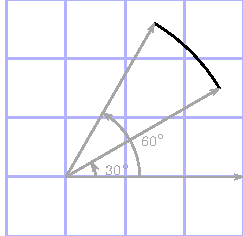
\includegraphics[width=\textwidth]{pstexam.pdf}
\end{column}
\end{columns}

\end{frame}

\subsection{TikZ}
\begin{frame}[c]\frametitle{\TIKZ 绘图}
PGF 和 Beamer 的作者都是 Till Tantau。Tantau 当初开发 Beamer
是为了准备 2003 年他的博士学位论文答辩,之后它在 CTAN 上流行开来。2005 年 PGF 从 Beamer 项目中分离出来,成为一个独立的宏包。而 \TIKZ 是 PGF 的前端,我们一般都是用 \TIKZ。

\begin{enumerate}
\item 配合恰当算法可以得到非常精确的结果;
\item 支持 \lstinline|PDFLaTeX| 与 \lstinline{XeLaTeX} 等;
\item 编译速度快,非常舒服的体验;
\item 学习难度大,绘图代码不直观更加复杂。
\end{enumerate}

\end{frame}

\begin{frame}[c,fragile]\frametitle{\TIKZ 示例}

\begin{lstlisting}
\begin{tikzpicture}
\draw [<->,thick] (0,2) node (yaxis) [above] {$y$}
    |- (3,0) node (xaxis) [right] {$x$};
\draw (0,0) coordinate (a_1) -- (2,1.8) coordinate (a_2);
\draw (0,1.5) coordinate (b_1) -- (2.5,0) coordinate (b_2);
\coordinate (c) at (intersection of a_1--a_2 and b_1--b_2);
\draw[dashed] (yaxis |- c) node[left] {$y'$}
    -| (xaxis -| c) node[below] {$x'$};
\fill[red] (c) circle (2pt);
\end{tikzpicture}
\end{lstlisting}

\begin{tikzpicture}
\draw [<->,thick] (0,2) node (yaxis) [above] {$y$}
    |- (3,0) node (xaxis) [right] {$x$};
\draw (0,0) coordinate (a_1) -- (2,1.8) coordinate (a_2);
\draw (0,1.5) coordinate (b_1) -- (2.5,0) coordinate (b_2);
\coordinate (c) at (intersection of a_1--a_2 and b_1--b_2);
\draw[dashed] (yaxis |- c) node[left] {$y'$}
    -| (xaxis -| c) node[below] {$x'$};
\fill[red] (c) circle (2pt);
\end{tikzpicture}

\end{frame}

\begin{frame}[c]\frametitle{关于我}

\begin{columns}
\begin{column}[c]{0.3\textwidth}
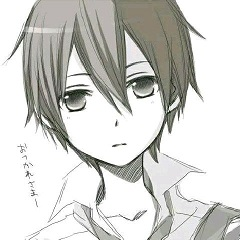
\includegraphics[scale=0.5]{author.jpg}
\end{column}
\begin{column}[c]{0.6\textwidth}
邓东升,就读于复旦大学经济学院(硕士),2010 接触 \LaTeX{},\LaTeX{} 用户以及爱好者,比较热衷于 beamer、绘图(TikZ)、模板设计等。2013 年与黄晨成共同建立 Elegant\LaTeX{},发布 ElegantBook 等模板。
\vskip2ex
\pbf{主页}:http://ddswhu.com/\\
\pbf{链接}:http://elegantlatex.org/\\
\pbf{邮箱}:ddswhu@outlook.com
\end{column}
\end{columns}


\end{frame}

\end{document}
